\documentclass[tikz]{standalone}

\usepackage{tikz}
\usetikzlibrary{automata}

\begin{document}

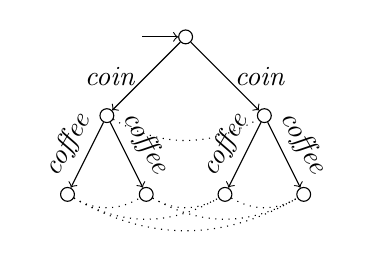
\begin{tikzpicture}
\tikzstyle{every state}=[
    draw,
    shape=circle,
    inner sep=1pt,
    minimum size=5pt,
    final/.style={double,minimum size=6pt},
    initial text=]
[auto,->]
\renewcommand{\a}[1]{\textit{#1}}
\node[state,initial] (r1) {};
\node[state,below of=r1,left of=r1] (r2) {};
\node[state,below of=r2,right of=r1] (r3) {};
\node[state,below of=r2,left of=r2,xshift=0.5cm] (r4) {};
\node[state,right of=r4] (r5) {};
\node[state,right of=r5] (r6) {};
\node[state,right of=r6] (r7) {};
\path[->] (r1) edge node[left] {\a{coin}} (r2) 
               edge node[right]{\a{coin}} (r3)
          (r2) edge node[above,rotate=60]{\a{coffee}} (r4) 
               edge node[above,rotate=-60]{\a{coffee}} (r5)
          (r3) edge node[above,rotate=60]{\a{coffee}} (r6) 
               edge node[above,rotate=-60]{\a{coffee}} (r7);

\path[dotted,bend right]
  (r2) edge (r3)
  (r4) edge (r5) edge (r6) edge (r7) 
  (r5) edge (r6) edge (r7)
  (r6) edge (r7); 
\end{tikzpicture}    
\end{document}